\documentclass[./A14_Report.tex]{subfiles}

\begin{document}
\chapter{Introduction}
\section{Overview}
\label{sec:overview}

The project aims to implement the \textbf{Embedded Zerotree Wavelet} algorithm
as a C library. It employs the well known \textit{Discrete Wavelet Transform}
as a tool for compression. The algorithm will be studied under several
operating conditions and demands, such as varying levels of
compression,``bit-budget'', etc

\subsubsection{The Basics}%
\label{sec:the_basics}

\textit{Data compression} is the science of representing any given information
in a compact form. A \textit{compression algorithm} by itself, refers to two separate 
algorithms. \textit{A compression algorithm} (takes $\alpha$ and generates $\alpha_c$) 
and a\textit {reconstruction algorithm} (takes $\alpha_c$ generates $\alpha$ or an approximation of $\alpha$), 
where $\alpha$ is a symbol. The compression technique is said 
to be \textit{lossless} if the reconstructed symbols are identical to the original symbols 
and it is said to be \textit{lossy} if the  reconstructed symbols are not identical to the original symbols.

\section{The transform coder}
\label{sec:the_transform_coder}

\begin{figure}[h]
    \centering
    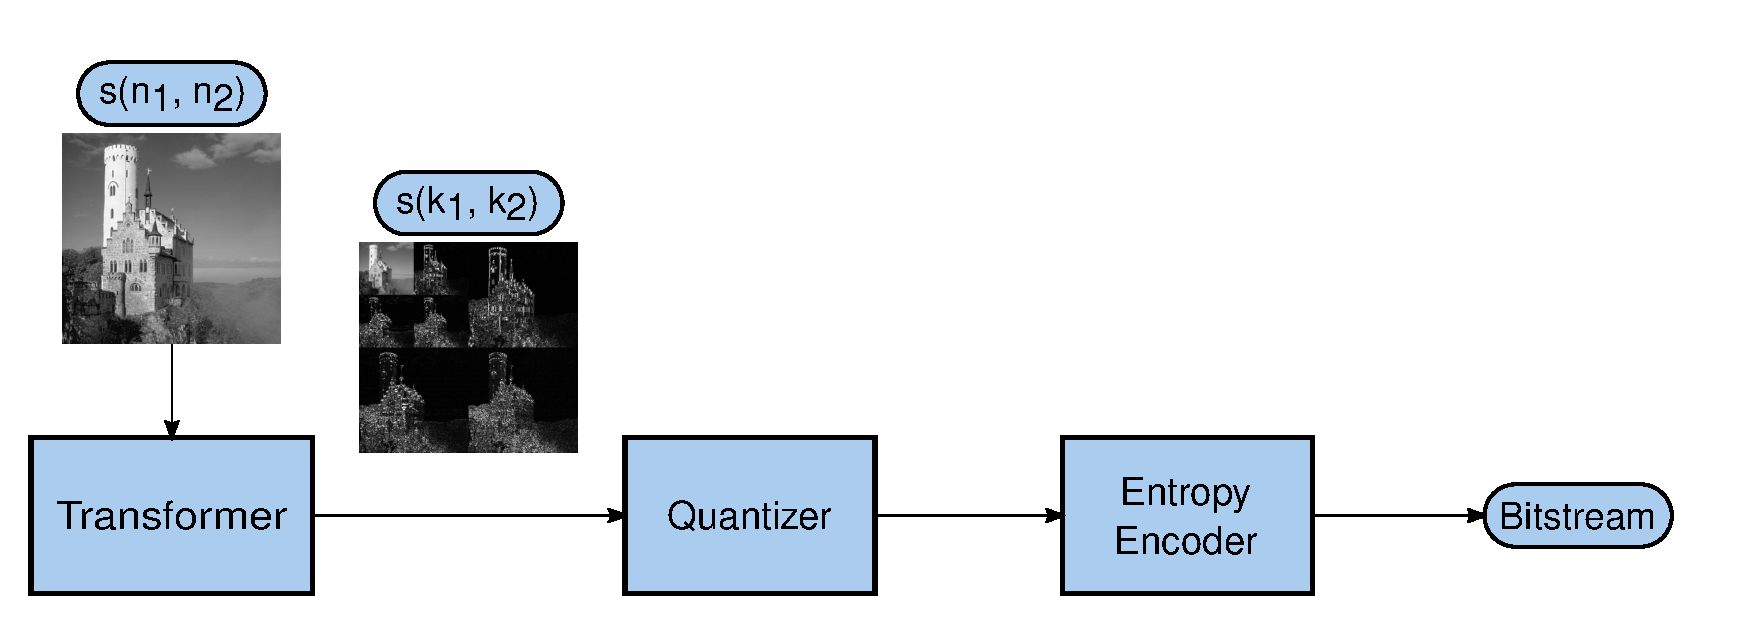
\includegraphics[scale=0.5]{../img/block-diag_shrunk.pdf}
    \caption{Transform coder: Generalised \cite{shap1993}}
    \label{fig:tcoder}
\end{figure}

A step-wise approach towards implementing this algorithm is taken, wherein
the each step is represented by a block in figure \ref{fig:tcoder}.

\pagebreak

\subsection{The transformer}
\label{sec:the_transformer}

The transformer performs a mathematical transform on the supplied image. The
transform must satisfy 2 key properties, namely:
\begin{itemize}
    \item Full invertibility
    \item Separability
\end{itemize}

A few transforms that satisfy these conditions are the Fourier transform, the
discrete cosine transform and the wavelet transform. Wavelet transform is used 
in this case, since it provides all the tools for performing multi-resolution analysis.

\subsubsection{Wavelets}%
\label{sec:theory_of_wavelets}

To overcome the shortcomings of traditional transforms such as the 
Discrete Fourier Transform (DFT), Discrete Cosine Transform (DFT), 
Short Time Fourier Fourier Transform (STFT), and Gabor Transform, 
the need for \textit{wavelets} arised. The fourier analysis provides key information 
in the frequency domain while fails to provide any information regarding the time domain.
The STFT and the Gabor Transform (STFT with Gaussian window function) provide concurrent
information about both time and frequency, but the window size is immutable.
Essentially, it is not possible to infer the exact frequency and the exact time of 
occurence of that frequency in the signal.

\par

The reason that wavelets are preferred for image analysis is due to the fact that it 
provides a hierarchical grading of the time and frequency information. The fact that low
frequency information exists for a longer period of time and the high frequency information
changes rapidly with time is exploited in wavelet analysis. In the case of image analysis, 
\textit{time} is equivalent to \textit{spacial area}. The phrase \textit{low frequency 
components exist in larger spacial area} indicates that the pixel values in that region
donot change significantly. Similarly, \textit{high frequency components} refers to the finer 
details which change rapidly in space. 
Higher temporal accuracy is required to observe the high frequency components and vice-versa.

\FloatBarrier
\begin{figure}[htpb]
    \centering
    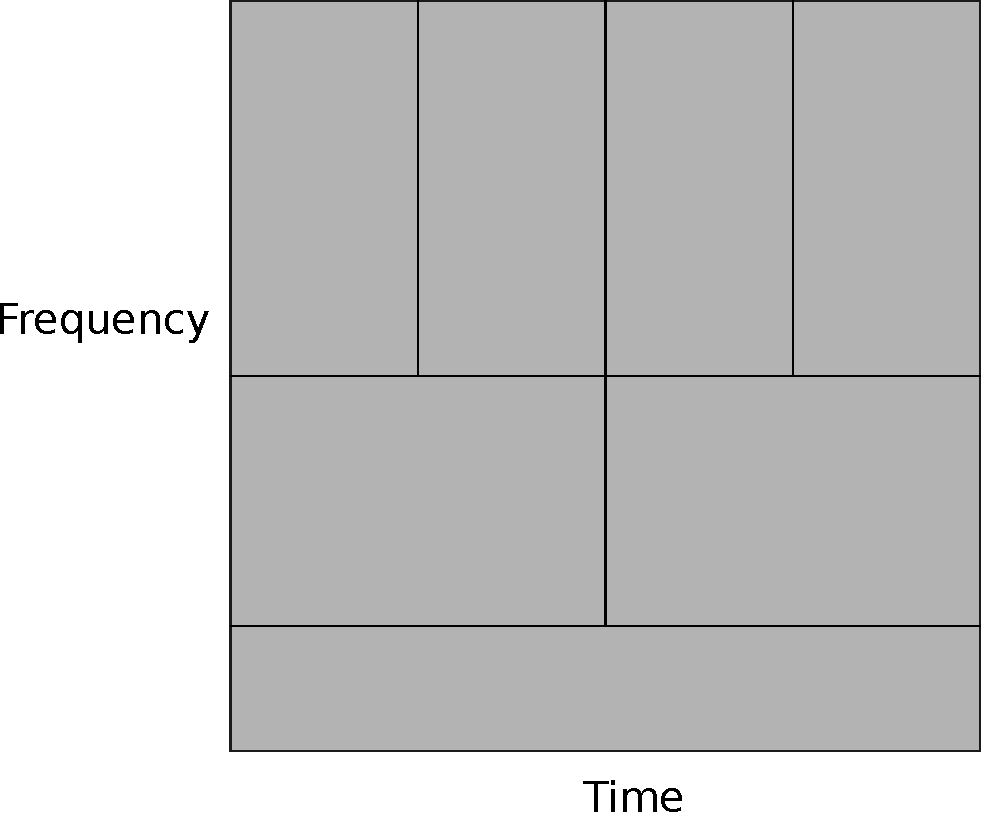
\includegraphics[scale=0.3, width=0.5\linewidth]{wt1.pdf}
    \caption{Multiresolution Analysis}%
    \label{fig:multiresolution}
\end{figure}
\FloatBarrier

\par

Performing wavelet analysis by utilizing a scalable and modulated window to calculate the
spectrum repeatedly provides the necessary collection of time-frequency representations 
of the signal. In this context, decreasing the scale is equivalent to focusing on higher
detail. \textit{Scaling} refers to increasing or decreasing the size of a portion of the signal 
by a factor and \textit{translation} refers to shifting a signal towards the right or the left.
The basis function which scales and translates to analyze other signals and generate
wavelets is called as the \textit{mother wavelet}. 

\par

There are numerous choices of wavelets that are available, for example, the \textit{haar, daubechies, 
coiflet, gaussian, etc} for performing wavelet analysis of images. 

\subsubsection{The Wavelet Transform}%
\label{sec:the_wavelet_transform}

The \textit{Continuous Wavelet Transform} (CWT) is mathematically represented by the
equation given below.

\[\gamma(s, \tau) = \int f(t)\cdot\psi^{*}_{s, \tau}(t)dt\]

\(f(t)\) is the signal to be decomposed into a set of basis functions \(\psi_{s,\tau}(t)\)
called the \textit{wavelets}. The new variables \(s\) and $\tau$ are the scale and translation
respectively. The wavelets generated by scaling and translating the mother wavelet
can now be mathematically represented as

$$\psi_{s,\tau}(t)=\frac{1}{\sqrt{s}}\cdot\psi \left (\frac{t-\tau}{s} \right)$$

The mother wavelet is scaled and translated to realize more orthogonal wavelets.
The issue with the CWT is that it brings in redundancy, and it's computation is time consuming.
To address these issues, the \textit{Discrete Wavelet Transform} was developed, 
which computes the transforms at various discrete samples.

Mathematically,

$$\psi_{j,k}(t) = \frac{1}{\sqrt{s_{0}^j}} \cdot \psi \left (\frac{t - k \tau_{0}s_{0}^j}{s_{0}^j} \right )$$

The wavelet transform is computed by calculating the inner product of the function with
a wavelet (mother wavelet after scaling and translating).
An important aspect here is that the DWT is not discrete in time, but the scale and 
translation parameters are incremented/decremented in steps \cite{valwav1999}. 
Further, it can be proved that implementing the wavelet transform as an iterative 
digital filter bank enables the subsampling property. This means that the signal is decomposed 
using filter banks, downsampled, quantized and encoded. 

\par

Applying the DWT on the images is equivalent to dividing the image into four different
\textit{subbands}. That is to say that, the wavelet based coding divides the image into hierarchical 
subbands critically subsampled. Each subband contains the wavelet coefficients and 
these coefficients interestingly represent a spacial area in the higher levels of subbands.

\FloatBarrier
\begin{figure}[htpb]
    \centering
    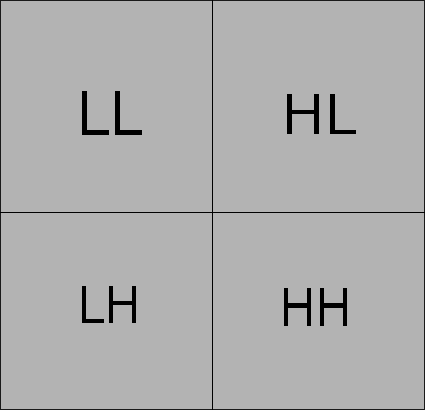
\includegraphics[scale=0.25, width=0.4\linewidth]{subband1.pdf}
    \caption{Image decomposition}%
    \label{fig:subband1}
\end{figure}
\FloatBarrier

\pagebreak

These four subbands are created by applying the digital filters in both the horizontal and vertical
directions. 
\begin{itemize}
    \item LL Subband: Realized by low pass filtering the image in both horizontal and vertical directions.
    \item HL Subband: Realized by high pass filtering the image in horizontal direction low pass filtering in vertical direction.
    \item LH Subband: Realized by low pass filtering the image in horizontal direction high pass filtering in vertical direction.
    \item LL Subband: Realized by high pass filtering the image in both horizontal and vertical directions.
\end{itemize}

These subbands are successively quantized for further compression. It is important to note that
every subband consists one-fourth of the total samples of a certain level of decomposition.
This process of successively decomposing the LL subband for image analysis is known as 
\textit{dyadic partitioning}.
Each of the subimages obatined in this manner can be filtered and subsampled until the
desired subband structure is obtained.

\FloatBarrier
\begin{figure}[htpb]
    \centering
    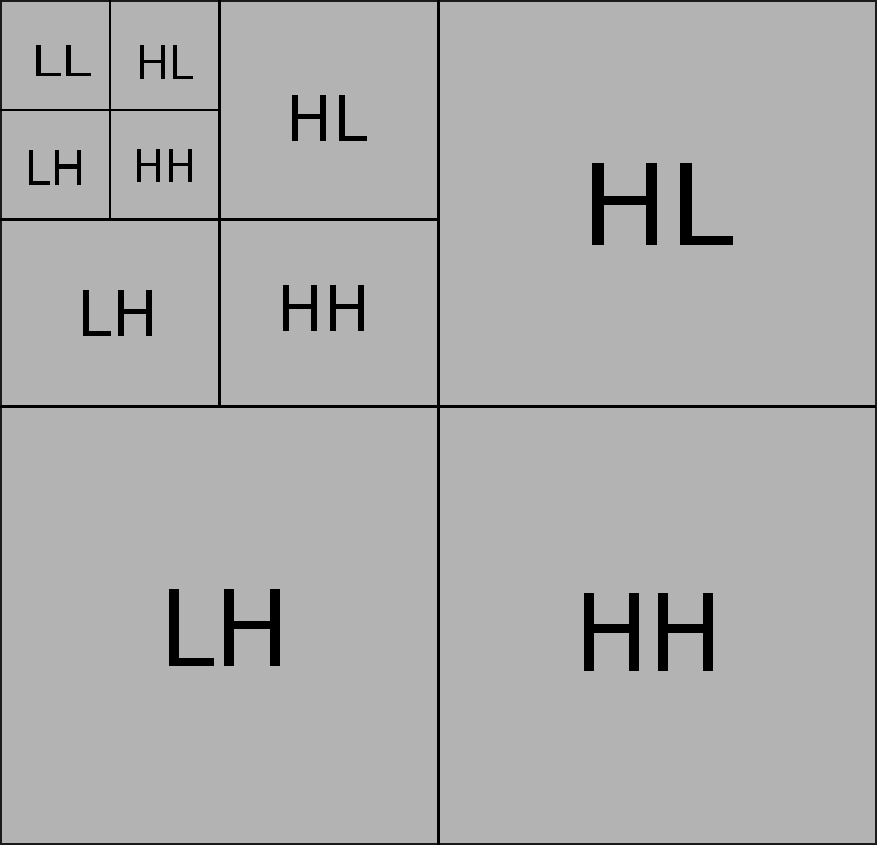
\includegraphics[scale=0.5, width=0.4\linewidth]{subband2.pdf}
    \caption{Multilevel subband decomposition}%
    \label{fig:subband2}
\end{figure}
\FloatBarrier

It is to be noted that when images are decomposed in this manner, most of the information
or the energy is concentrated in the lower subband (mostly LL subband), which confirms 
that low frequency components contain the maximum information of that spacial area.
Generally the LL subband is a low resolution and inexpensive approximation of the original
image, while the other subbands contain the finer details (horizontal, vertical, and diagonal)
that can be added.

\subsection{The quantizer}
\label{sec:the_quantizer}

The wavelet transformed coefficients are to be quantized to produce the \textit{bitstream}.
All information loss happens during the quantization stage.
The coefficients are passed through a midtread quantizer to obtain the initial 
reconstructed value of the coefficient, which is $\pm 1.5$ times the initial threshold value. 
To achieve higher precision of reconstructed values, refinement is done by encoding the
quantized difference value of the coefficient and it's reconstructed value and using it
for final reconstruction.
% \subsection{The entropy encoder}
\end{document}
